
\section{UTKAST: ikke les}


Som med animasjon kan lyd både virke for og i mot sin hensikt. Horanger og Nielsen fant ut under testing av nettsider at ungdommer og voksne fant kvitre og kime lyder var irriterende, men at de appellerte til barn. 

Sammen med animasjoner kan lyder i programvare være effektive til å gi brukeren tilbakemelding på en handling. Eksempelvis kan lyder brukes til varsle brukeren om at de har gjort et feil valg \cite{}, men som med animasjoner vil for mange lyder og uventede lyder være distraherende og irriterende. Nielsen og Loranger fant 




I prototypen ønsker animasjonen å vise hva som skjer,  ved at symbolet beveger seg fra opprinnelige posisjon til set

I Sono Flex dukker symbolet bare opp i setningslisten.

I symboltabellen er det 3 forskjellige typer. Man har 
ordsymbol, kategorisymbol og navigasjonssymbol. Et ordsymbol representerer selvsagt et ord og vil legge seg i listen sammen med andre ord som vil bli 

For å vise hva som skjer, fremfor at det bare skjer. I den eksisterende løsningen Sono Flex var det ingen for animasjoner. Slik at når brukeren trykte på en knapp, skjedde responsen umiddelbart. Man kan si at animasjonene skal representere det som skjer med dataen. Eksmepelvis hvis brukeren trykker på en knapp 


//tre ulike knapper
    //Trykk på knapp
    //neste side
    //Organisasjon



Det vil derfor være viktig at animasjonene som er implementert gir verdi til applikasjonen fremfor å distrahere.

Det vil derfor være viktig å finne ut om animasjonene gir noe verdi 

Interaksjonsdesigneren Nielsen har gjort flere undersøkelser på hvordan en skal få optimal brukervennlighet på webapplikasjoner. 

Animasjoner i programvare og nettsider blir ofte snakket om i negative ordlag fordi de

for det de ofte blir brukt overdrevet mye og er u

Animasjoner blir ofte sett på som en distraksjon når det blir brukt i applikasjoner for det de fjerner fokuset fra det som er viktig. Som 


For å kunne sjekke hvordan animasjon påvirket et barns evne til å samhandle med applikasjonen, måtte de ble implementert.  

//visualiserer at symbolet går fra griden til output, hjelper barnet
// Vanskeligheten med å skaffe empirisk data


Dataanimasjon, animasjonsfilmteknikk som gjør bruk av elektronisk databehandling for å skape illusjon av bevegelse, har fått en svært sentral plass innenfor reklamefilm og fjernsyn. Her har utviklingen gått fra enkle todimensjonale tegninger til avansert 3-D-animasjon som ikke kan fremstilles på andre måter enn med datamaskin.

Ifølge Store norsk leksikon defineres animasjon som levendegjørelse, besjeling, oppmuntring, tilskyndelse. 


Applikasjonen tilbyr flere animasjoner som brukeren kan velge mellom, enten alene eller flere i kombinasjon. Noen animasjoner kan ikke være operative samtidig ettersom det vil føre til konflikt. 

\subsection{Fade in, fade out}

Gjør rede for og forklar de ulike animasjonen

\section{Navigasjon}
Gjør rede for og forklar de forkjellige navigasjons hjelpemidlene

\section{Personlig tilpasning}
Forklar hvordan applikasjonen legger til rette for brukeren.
    - Temaer, forkjellige farger, lyder, 
    - Bruker kan velge hvilke animasjoner som ønskes og hurtigheten på dem.
    
\section{Lyd}
    Gjør rede for de ulike lydene.

\chapter{Dette er bare utkast og stikkord}

Rapporten vil ikke gi noen videre beskrivelse av C-Sharp, derimot vil WPF bli forklart.


\section{Teknologier}

Øyesporingsenheten beskrevet i kapittel  krever at systemet kjører på operativ systemet Windows og APIet som det leveres enheten leveres med,  fungerer kun i programmeringspråkene C-Sharp og C++. Med dette som utgangspunkt ble resten av teknologivalgene er basert på anbefalinger fra dokumentasjonen og tidligere erfaring. 


\begin{description}
  \item[IDE] Visual Studio
  \item[Rammeverk] .NET
  \begin{description}
     \item[Programmeringspråk] C\#
     \item[Grafikk] Windows Presentation Foundation 
\end{description}
  \item[Versjonskontroll] Git (BitBucket)
\end{description}


Fitzergald key, personliggjør keyboardet med farger. Viktigste er at det er konsistent


For å kunne bruke symboler som en kommunikasjonsform kreves det at brukeren har mulighet til samhandle med dem. For å få til dette brukes det en øyestyringsenhet koblet til en datamaskin som fanger opp brukerens pupill bevegelser. På den måten erstatter øyene den vanlige musepekeren.

\subsubsection{Kalibrering}

Første gang en kobler øyestyringsenheten til maskinen, anbefales det at brukeren gjør en oppmåling og kalibrering for mer presis øyesporing. Oppmålingen innebærer at personen måler størrelsen på skjermen - kalibreringen at det brukeren bes om å følge en prikk som traveserer skjermen. Ettersom dette vil gi øyestyringsenheten et referansepunkt. Prosessen er kun nødvendig første gang for gjeldene bruker. 

Dette gir tilgang på deres application programming interface (API), herved referert til som Tec API. Tec API gjør funksjoner og informasjon fra sporingsenheten tilgjengelig. 


The Tobii Eye Control API provides two alternative access points: a .NET assembly and a C dynamic-link library. Both alternatives
give the developers of eye controlled applications access to the functionality of the Gaze Interaction Server. The .NET API also
contains specialized interaction support for common user interface frameworks such asWindows Presentation Foundation
(WPF) andWindows Forms. The C interface, called MPACI, provides backward compatibility with older Tobii products such as
the MyTobii software.


\subsection{Systemkrav}

\subsection{Nøkkelfunksjoner og konsepter}

\section{}



Første gang en kobler til må en gå igjennom ett oppsett. Dette innebærer måling av den aktuelle skjermen som brukes og en kalibrerings rutine. For å oppnå nøyaktig øyesporing.  

For en førstegangsbruker av enheten anbefales det å gjøre en kalibrering, for optimal opplevelse. Informasjonen


Øyestyringsenheten som er illustrert i figur \ref{fig:tobiiPc}  . Denne



\subsection{Utfordringer}

En utfordring ved øyesporing er blunking. Blunking er et er en kortvarig sammentrekning av øyelokket, noe som gjør at øyet ikke vil gi refleksjon som kamera kan fange, og derfor ikke ha koordinater på hvor brukeren ser. Dette løses under analysen. Ved at og bruke koordinatene og øyets hurtighet før øyelokkene trakk seg sammen kan man ekstrapolere seg fram til en tilnærmet korrekt fiksering. 


\subsection{Tobii Software Developer Kit}
\label{subsec:blikk}

Sammen med Tobii PCeye go følger det med programvare for å kontrollere applikasjoner som bruker sporingsenheten. De ulike komponentene er beskrevet nedenfor. I denne rapporten vil kun førstnevnte være relevant. Ettersom applikasjonen er spesialisert til blikkinteraksjon og ikke er en standard Windows applikasjon.

\subsubsection{Blikk interaksjonsserver}
en sentral HUB som tilbyr klient applikasjoner øyesporingsdata. 

\subsubsection{Blikk interaksjons innstillinger}
Et kontrollpanel for interaksjons innstillinger og oppgaver relatert til øyesporing.

\subsubsection{Windows Kontroll}
Tilbyr blikk interaksjon for standard Windows applikasjoner, ergo vanlige applikasjoner som ikke er laget for øyesporings interaksjon.


\subsection{Blikk Interaksjonsserver}

Blikk interaksjons-serveren er som nevnt i seksjon \ref{subsec:blikk} en HUB for programvaren, eller kjernen. Hovedformålet til denne komponenten er å samhandle med Øyesporingsenheten og tilby interaksjonsfunksjonalitet for å kontrollere Windows baserte applikasjoner som vil bruke sporingsdata. I tilegg er det denne komponenten som tar seg av kalibrering, sporingsstatus - samt bruker og applikasjons innstillinger.


\section{eXtensible Application Markup Language} 
 
 WPF bruker eXtensible Application Markup Language (\gls{XAML}), som er et XML-basert språk til å definere og kombinere ulike grensesnittelementer. Figur \ref{lst:myLabel} viser hvordan et vindu med en knapp er definert i XAML. Resultatet kan ses i figur \ref{fig:xamlButton}.  
 
 
For å kunne samhandle med de grafiske objektene definert i XAML filen opprettes det alltid en tilhørende kodefil sammen med denne. Kodefilens formål er å ta seg av data og logikk for å ha et klart skille mellom utseende-spesifikk kode og oppførsel-spesifikk kode. For eksempel så vil en knapp sitt utseende og plassering bli definert XAML filen, mens hvordan data blir påvirket av interaksjon med knappen blir definert i den tilhørende kodefilen. 
 
WPF oppfordrer til å skille mellom utseende spesifikk kode og oppførsel-spesifikk kode ved at grafiske elementer skrives i XAML og interaksjonen  kun brukes til generere  
XAML brukes til å generere brukergrensesnitt,  
,Hver XAML-fil har en tilhørende kode-fil for håndtering av hendelser og oppførsel. Dette gjør at koden har et klart skille mellom utseende-spesifikk kode og oppførsel-spesifikk kode. Den tilhørende kode-filen til XAML koden beskrevet i kodesnutt \ref{lst:myLabel} er vist i kodesnutt \ref{lst:backbutton}. Ved å trykke på knappen bildet vil metoden button\textunderscore Click i kodefilen bli kalt og en dialogboks vist til brukeren. 
 
 
 
 //Usikker på om dette skal bli med
  For at en bruker skal kunne utføre kommandoer og hente data gjennom et view, brukes det i WPF, databindings uttrykk som blir evaluert opp mot viewets gitte datakontekst. I MVVM vil datakonteksten være satt til viewmodellen. Det vil si som figur \ref{fig:mvvm} viser, at alle former for kommandoer, notfikasjoner og databinding skjer gjennom viewmodellen. Et view skal kun forholde seg til en viewmodel, altså et en-til-en relasjon\cite{.   
 

Mens viewet bestemmer hvordan applikasjonen skal se ut, så bestemmer viewmodellen hvordan funksjonaliteten skal være \cite{THEM6:online}. Det er i viewmodellen at egenskaper og kommandoer som viewet kan binde seg opp mot er implementert. Når data  da endres vil view bli varslet og oppdatert deretter(Notified i figur \ref{fig:mvvm}) . På samme måte vil viewet kalle på viewmodellen om at en kommando må kjøres hvis for eksempel en bruker trykker på en knapp. Det er også Viewmodellen sitt ansvar og koordinere interaksjoner med viewet med de modellene som trengs. Det vil si at viewmodellen kan eksponere modellen direkte til viewets slik at bindingen kan skje direkte mellom dem. Samtidig kan viewmodellen også manipulere data fra modellen , som for eksempel å kombinere to verdier. Eksempel kan være å sette sammen fornavn og etternavn fra en Person modell. Mens forholdet mellom View og Viewmodellen typisk er en-til-en, så vil ViewModellen ha en en-til-mange relasjon.  




\subsubsection{Innlesning}


For å kunne skrive med skrivebordet er det nødvendig at det er fullt opp med ord og symboler. For å gjøre dette blir metoden texttt{GetInitialPages} vist i figur .. kalt fra konstruktøren. Denne metoden kaller så igjen på metoden GetCategory("Frontpage") i klassen \texttt{Dataservice} vist i figur ... Grunnen til at ViewModellen ikke kun direkte henter symbolene er fordi de er lagret på et tekstdokument. Så for å separere data fra presentasjon- og forretningslogikk så brukes det et data tilgang lag i mellom. For å gjøre om tekstfilen til strukturerte data bruke datatjenesten klassen TextParser til å tolke den. 


\subsubsection{Data og innlesning av dem}

Programvaren skal strebe etter å kunne tilby brukeren ordene han har lyst å bruke. Noe som kan være utfordrende med tanke på at et barns vokabular allerede i alder av 5 år kan være opp i mot XXXX ord. Med tanke på hvilke ord som er i vokabularet vil variere  fra person til person så må programvaren ha en god del mer enn dette. I tillegg må også programvaren tilby et bilde for vært av ordene. 

En naiv fremgangsmåte for å lage brikkene er å statisk initialisere hver brikke med et ord og bilde. Problemet med dette er først og fremst at XAML koden blir unektelig lang som følge av at en må skrive en knapp for vært tilfelle. Den at en også må inn i koden for å gjøre endringer eller legge til nye ord, er ugunstig ettersom det er en ressurskrevende prosess. Løsningen på dette var å oppbevare alle ordene i en separat fil for å skille mellom brukergrensesnitt og data. For at maskinen skulle ha mulighet til å lese dataene ble de lagret i JavaScript Object Notation(JSON) format. JSON er ifølge sine egne nettsider \cite{JSON7:online} et lettvekt data-utvekslings format. Som er lett for mennesker å lese og skrive og det er lett form maskiner å tolke og generere. Kode \ref{listing:jsonfile} viser et utdrag fra json filen hvor ordene og stien til bildet som representerer ordet, er lagret. Filen består i en liste med JSON objekter som har attributtene Name og Image. Der Name er ordet og image er stien til symbolet. Dette er bare et lite utdrag fra filen og viser kun det som ville tilsvart fire brikker i programvaren. Det første objektet "I" er et ord, mens de tre neste er kategorier. Hver kategori består av flere ord. Ordene som tilhører en kategori er lagret i en egen fil i en mappe med samme navn. Figur \ref{jsonstructure} viser strukturen på filene, der hver kategori har sin egen mappe. Dette gjør at data hentes "just-in-time". Det vil si at istedenfor at ordene ligger i minnet til enhver tid, så hentes de kun når ved behov. Eksempelvis hvis en bruker trykker på kategorien "Food and Drink" så vil ordene hentes fra "FoodAndDrink.json" i mappen "FoodAndDrink". Noe som sparer på minnet, men som kan forringe kjøretiden. For når det er snakk om så store mengder data som alle ordene ville gitt, er det ikke gunstig å bevare dem i minnet. 


\begin{listing}[ht] 
\inputminted[fontsize=\footnotesize, frame=lines,framesep=2mm,baselinestretch=1.2,bgcolor=lightgray,linenos]{json}{Code/JSONfile.json} 
\caption{Utdrag fra filen som inneholder ord og sti til bilde som representerer det i JSON format} 
\label{listing:jsonfile} 
\end{listing} 
 
 
 \begin{figure}[ht!] 
\centering 
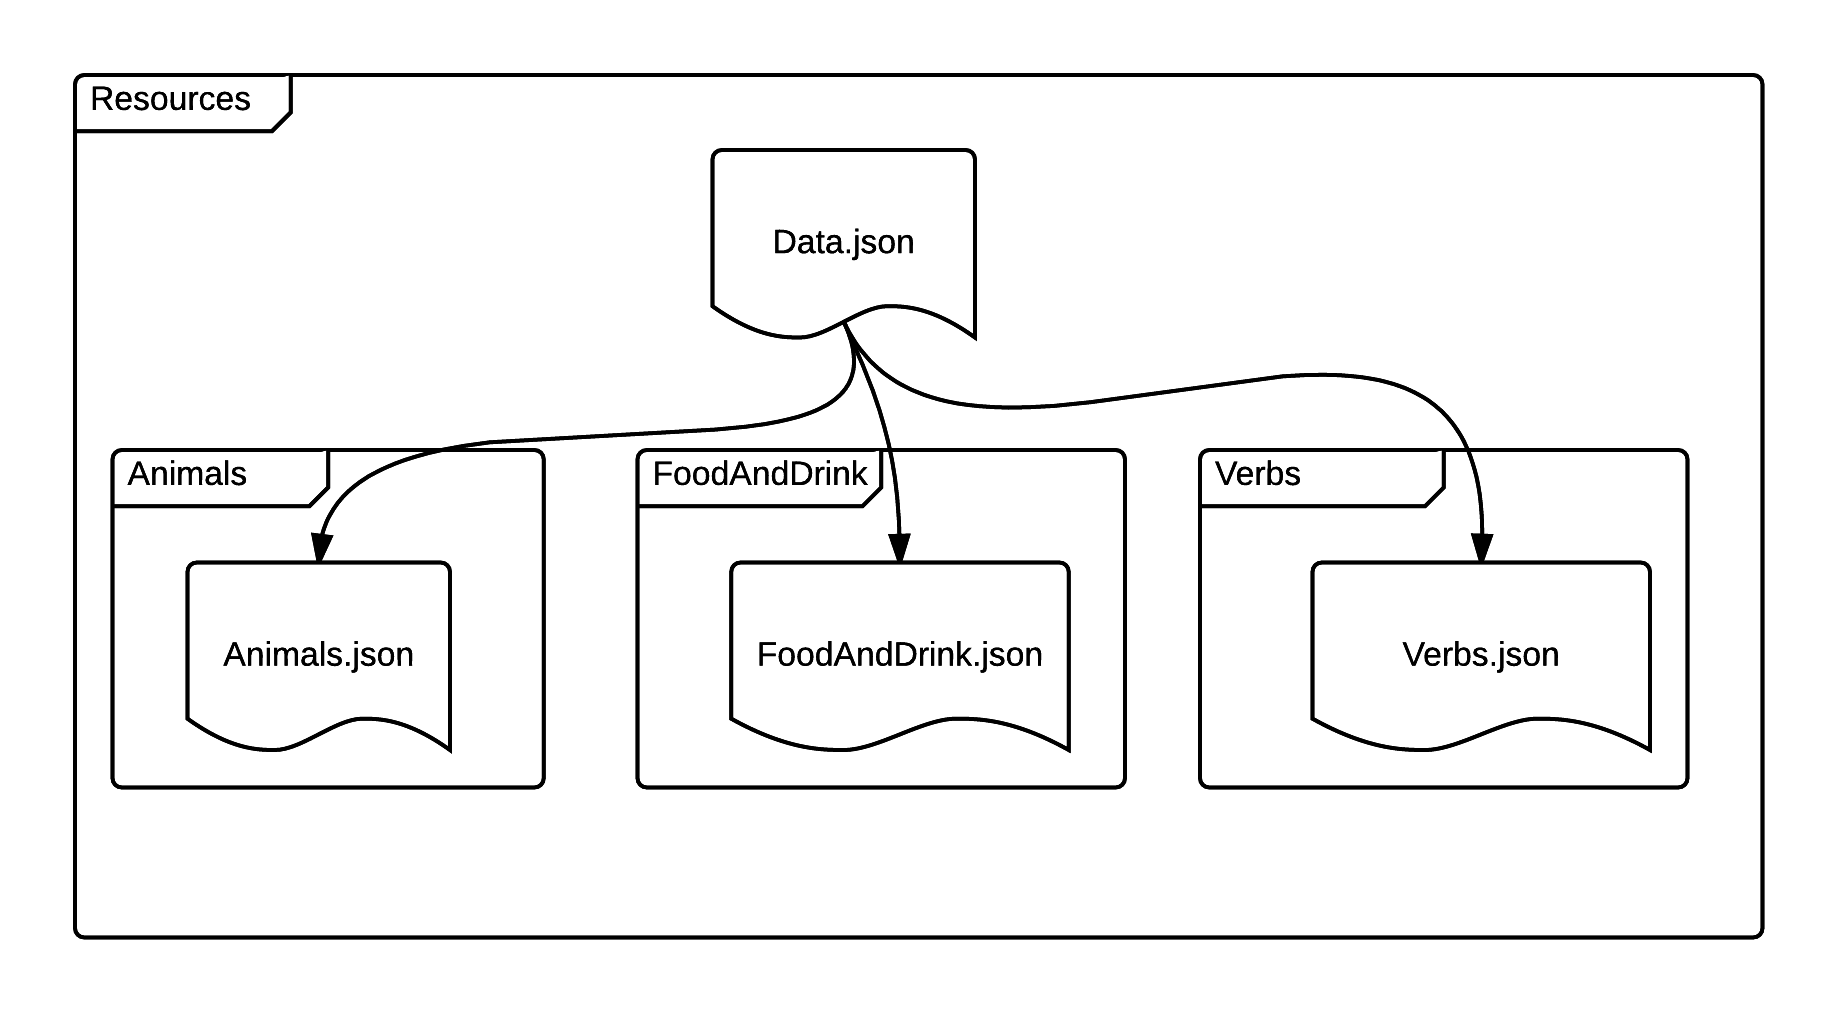
\includegraphics[width=100mm]{JsonStructure} 
\caption{Bilde av dokumentet hvor de ulike symbolene er registrert} 
\label{fig:jsonstructure} 
\end{figure} 


For å kunne ta i bruk objektene definert i tekstfilen må de tolkes fra JSON format til .NET objekter. Denne prosessen, å trekke ut datastrukturer fra bytes, kalles deserialisering. For å gjøre dette har vi brukt et tredjeparts rammevekt kalt JSON.net \cite{Json.0:online}. Det finnes en innebygd funksjon i .NET kalt DataContractJsonSerializer \cite{DataC3:online} som også greier å deserialisere et JSON dokument. Grunnen til at JSON.NET ble brukt er fordi i dette biblioteket er det mulighet for å automatisk deserialisere en helt liste av JSON objekter til .NET liste uten å manuelt måtte legge inn objektene. Ifølge utviklerens egne nettsider skal rammeverket være 50 prosent kjappere enn DataContractJsonSerializer, men ytelsen er avhengig av hvilke datasett som brukes, og har ikke vært en faktor i avgjørelsen. 


\begin{listing}[ht] 
\inputminted[fontsize=\footnotesize, frame=lines,framesep=2mm,baselinestretch=1.2,bgcolor=lightgray,linenos]{csharp}{Code/JSONparser.cs} 
\caption{Koden som konverterer JSON filen til en IList} 
\label{listing:JsonParser} 
\end{listing} 


Koden i figur \ref{listing:JsonParser} deserialiserer JSON dokumentet om til en dataliste. Fra linje 5 til 12 skrives teksten fra filen over til en streng som kan manipuleres i koden. På linje nummer 14 blir strengen konvertert til et dataobjekt. Det at dokumentet blir gjort om fra streng til et komplekst objekt på kun en linje viser noe av styrken til json.NET. 

\begin{listing}[ht] 
\inputminted[fontsize=\footnotesize, frame=lines,framesep=2mm,baselinestretch=1.2,bgcolor=lightgray,linenos]{csharp}{Code/CategoryModel.cs} 
\caption{Category modellen har egenskapen navn og en liste over alle sidene som utgjør alle symbolene som hører til i kategorien} 
\label{listing:CategoryModel} 
\end{listing} 


\subsection{Teksttolker}

Under utviklingen ble det bare lagt inn tilfeldige ord i prototypen, men ettersom prototypen begynte å bli ferdigstilt var det behov for et større utvalg ord og symboler Det ble derfor gitt tillatelse av Tobii Dynavox til å ta i bruk det samme bildene som de bruker i deres programvare. Denne bildepakken heter SymbolStix og har gir tilgang på cirka 16 000 symboler og er levert av et eksternt selskap som heter n2y \cite{n2y}. 

\begin{itemize}
\label{itm:egenskaper}
\item Symbol ID
\item Dato oppdatert
\item Dato laget
\item Kategori Navn 
\item Filnavn
\item Filsti
\item Ord
\item Synonymer
\item Tysk, nederlandsk, norsk, svensk, dansk, engelsk, spansk, italiensk, fransk, portugisisk.
\end{itemize}


Sammen med bildepakken fulgte det med et dokument som hadde en beskrivelse av vært symbol. For vært symbol var egenskapene beskrevet i liste \ref{itm:egenskaper} tilgjengelig. Disse var strukturert med at de kom i rekkefølge og hadde tilde notasjon(tilde) for å skille mellom dem. Dette gjorde at det var mulig å implementere en løsning for å gjøre dem om til datastrukturer. I tillegg til å tilby det samme som JSON dokumentet, ord og bildesti, så har den også ordets kategori og synonymer for ordet. Det er også mulighet for å få ordet på flere språk og synonymer til de ulike språkene. Noe som åpnet for flere muligheter, men for å få til dette, måtte det legges til en annen form for innlesing av data ettersom dokumentet ikke var lagret i JSON format og I motsetning til å dele opp symbolene opp i separate dokumenter basert på hvilken kategori de tilhørte, så var alle deklarert på et dokument. Så for å kunne løse dette sto vi mellom å lage et skript som oversatte dokumentet til JSON format eller lage en alternativ innlesning. Å omgjøre det fra tekst til JSON hadde vært mulig, problemet med dette er at dokumentet utsatt for oppdatering. Så hver gang dokumentet blir forandret må oversetting gjøres på ny. Så det ble da bestemt for å implementere en teksttolker. 

Tekstolkeren er er mer kompleks enn JSON tolkeren. Hovedsaklig fordi det ikke finnes noe biliotek som automatisk tilegner egenskaper til symbolene. Egenskapene blir derfor gitt til vært symbol etterhvert som de blir lest inn. En annen utfordring var som tidligere nevnt at alt befant seg på et dokument som da totalt utgjorde 16 000 linjer med beskrivelse av symbolene. Slik at hvis en skulle ha brukt samme fremgangsmåte som med JSON parseren å kun lest inn for den gitte kategorien. Så hadde en i verste fall måtte ha lest 16 000 linjer med tekst. Dette er ikke gunstig. Dokumentet har flere kategorier og symboler som ikke er nødvendig for barn, blant annet egne kategorier som eksempel Brasil, hebraisk og sveitsisk. Det er også flere kategorier som kunne vært greit å ha, men som ikke prioriteres som blant annet kategorier om kjendiser og en egen om amerikanske byer. Det ble derfor bestemt å kun velge kategorier som var nødvendige.

\begin{figure}[ht!] 
\centering 
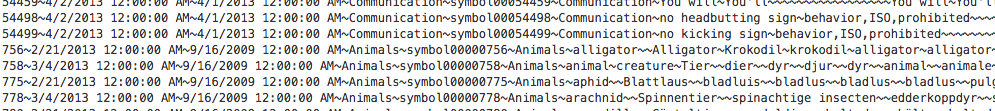
\includegraphics[width=100mm]{datafil} 
\caption{Bilde av dokumentet hvor de ulike symbolene er registrert} 
\label{fig:dok} 
\end{figure} 


\subsection{Modellene}

Modellene i MVVM mønsteret enkapsulere forretningslogikk og data. Der forretninslogikk er definert som all applikasjonslogikk med tanke på innhenting og håndtering av applikasjonsdata for forsikre seg om at data er konsistent og validering er pålagt. Bruk av modeller skal hjelpe til med å maksimere gjenbruk.

I applikasjonen er det flere modeller, men det som blir brukt mest er Symbol modellen. Denne representerer alle data i symboltabellen. Der det blant annet er et bilde og et ord som representerer dette bildet. Den har også egenskaper som forteller om hvilken type knapp det er, altså navigering,kategori eller ord. Hvilken knapp det er vil påvirke hva som skjer når en bruker interagere med denne.



\section{Utvikling}  
 
 
I seksjon \ref{sec:utgangspunk} ble teknologien som ble brukt til å utvikle prototypen diskutert. I denne seksjonen vil arkitektturen og de viktigste utviklingsdetaljene  bli drøftet.  
 
 

 
 \subsection{Skrivebordet}
 
KeyboardViewModel og KeyboardView utgjør sammen det som blir kalt skrivebordet. Skrivebordet er den delen av programvaren som tilbyr hovedfunksjonaliteten, å la en bruker kunne skrive setninger. For å gjøre dette så må er det en del viktig elementer som må være tilstede. Man kan si at skrivebordet skal være en digital representasjon av det klassiske tastaturet. Der det er ord med symboler istedenfor bokstaver, og trykk skjer ikke ved fysisk trykk, men ved å se på knappen over en periode. Utenom dette skal funksjonaliteten være mye den samme. De mest nødvendige funksjonene som å kunne viske og bygge setninger må ihvertfall være tilstede. I tillegg må prototypen ha mulighet for å kunne presentere setningene som lyd. 

\begin{figure}[ht!] 
\centering 
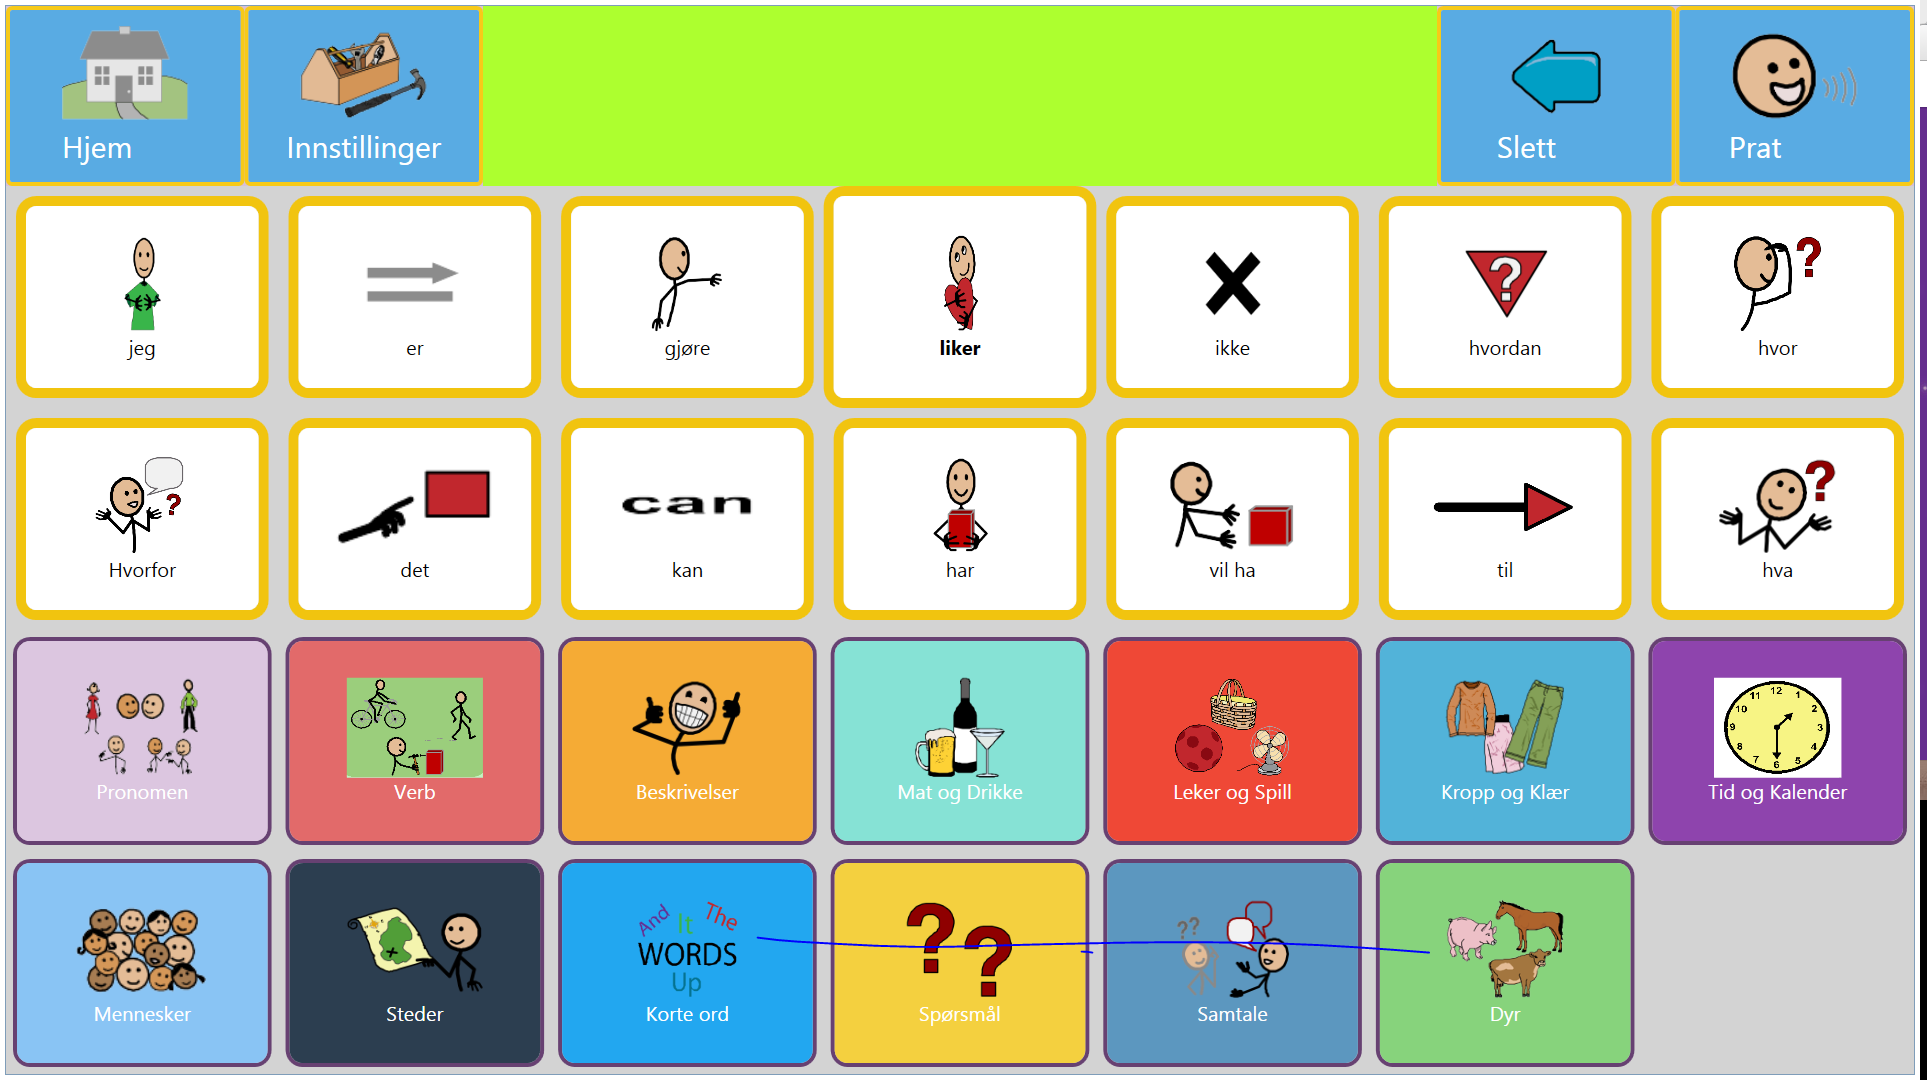
\includegraphics[width=100mm]{skrivebord} 
\caption{Skjermdump av skrivebordet i prototypen} 
\label{fig:skrivebord} 
\end{figure} 
 


\subsection{Arkitektur} 
 
 
Figur \ref{fig:arkitektur} viser et forenklet bilde over hvordan klassene i kodebasen er koblet sammen. Med forenklet så menes det at flere hjelpeklasser og tredjeparts bilioteker er med i diagrammet. I tilegg så har ikke Views blitt tatt med i diagrammet, men for hver ViewModel så er det View som representerer det.  
 

\begin{figure}[ht] 
\centering 
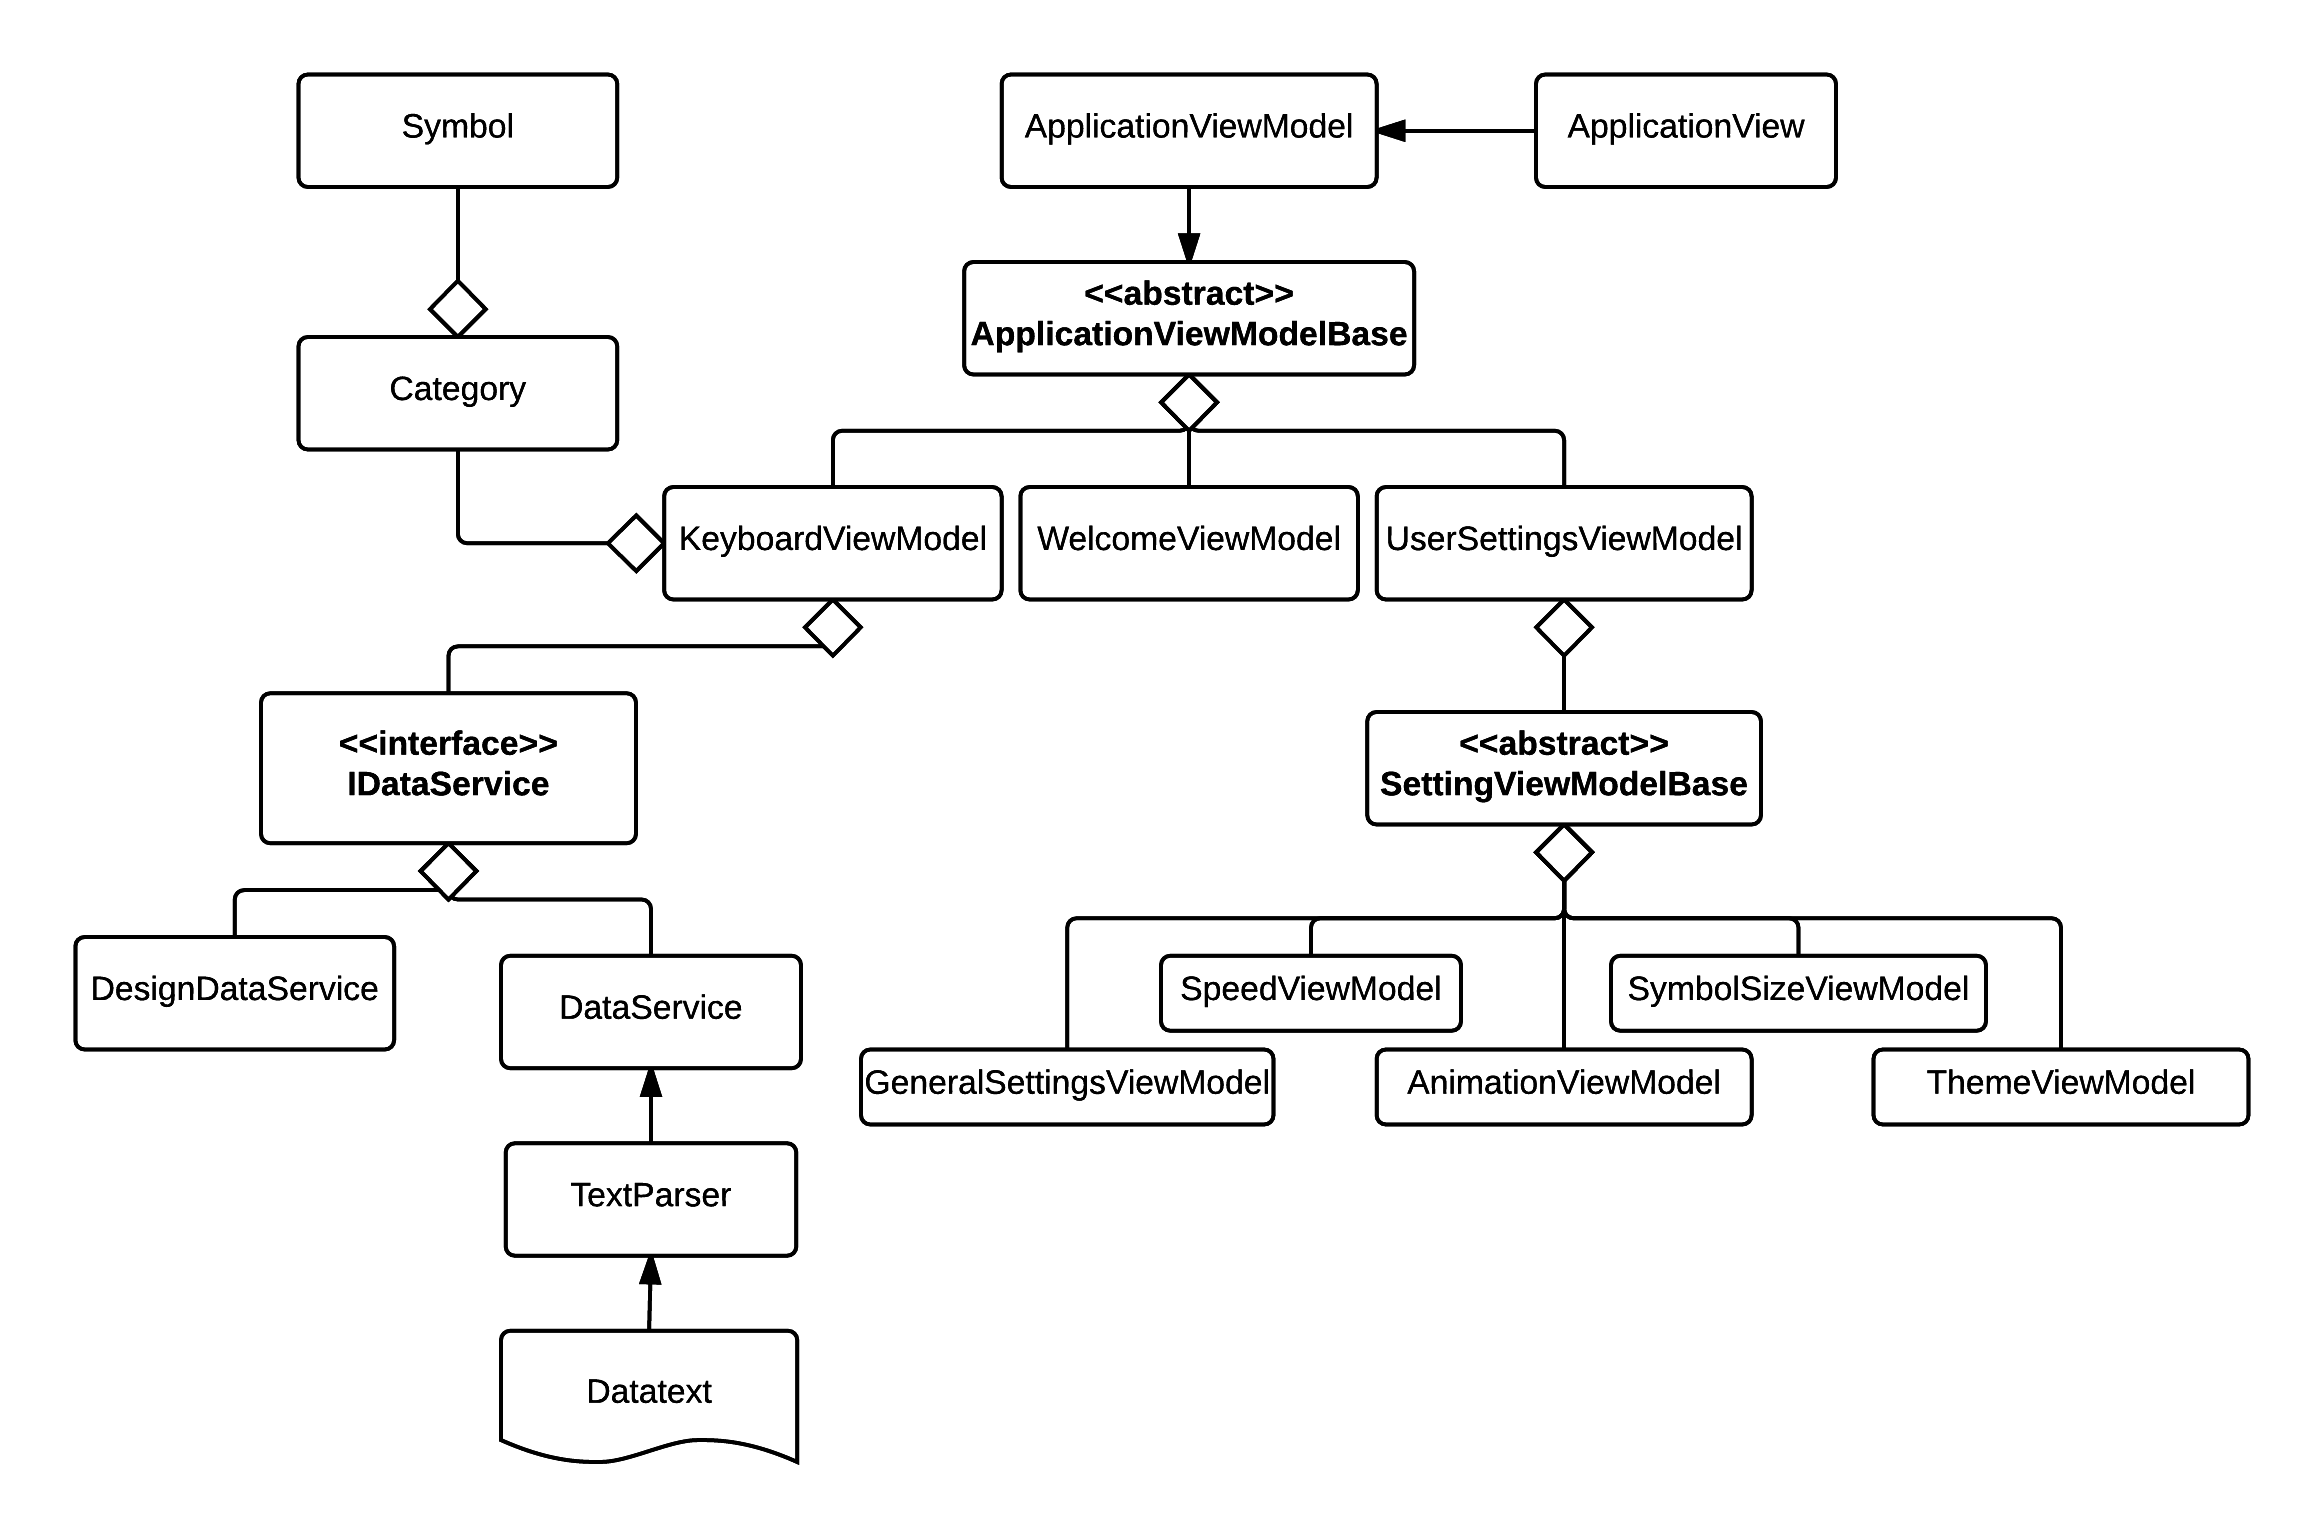
\includegraphics[width=140mm]{Arkitektur} 
\caption{Figur som viser et overordnet bilde av hvordan de ulike klassene henger sammen} 
\label{fig:arkitektur} 
\end{figure} 
 

ApplicationViewModel er vinduet som åpnes når programmet startes. Denne klassen fungerer som en kontainer for applikasjonen og bestemmer kun applikasjonsvinduets størrelse og navigasjon mellom de andre viewmodellene Keyboard, Welcome og UserSettings.  
 
 

\begin{listing}[ht] 
\inputminted[fontsize=\footnotesize, frame=lines,framesep=2mm,baselinestretch=1.2,bgcolor=lightgray,linenos]{xml}{Code/ApplicationContainer.xml} 
\caption{Utdrag fra kode som viser hvordan kontainer er satt opp} 
\label{listing:Kontainer} 
\end{listing} 
 
 
\begin{listing}[ht] 
\inputminted[fontsize=\footnotesize, frame=lines,framesep=2mm,baselinestretch=1.2,bgcolor=lightgray,linenos]{csharp}{Code/CurrentApplicationView.cs} 
\caption{Utdrag fra kode som viser hvordan kontainer er satt opp} 
\label{listing:CurrentAppView} 
\end{listing} 
 
 
 
Figur \ref{listing:Kontainer} viser hvordan ContentControl elementet i ApplicationView fungerer som en kontainer ved at innholdet er bundet til egenskapen CurrentViewModelBase. Som vil si at innholdet i ContentControl vil basere seg på hva som er satt som CurrentViewModelBase i ApplicationViewModel. Figur\ref{listing:CurrentAppView} viser hvordan denne egenskapen er implementert i Viewmodellen. Utfra koden så kan man se at til forskjell fra viewet, som hadde en referanse til egenskapen, så er det ingen direkte referanse fra viewmodellen til viewet. Dette er for å følge prinsippet til MVVM om at viewmodellen ikke skal ha noe kjennskap til Viewet, som gjør koden løs koblet(les: loose coupled). Men siden dette er en verdi som antakeligvis vil endre seg i løpet av kjøretiden er det nødvendig at Viewet blir gjort oppmerksom på forandring. Dette skjer ved å avfyre RaisePropertyChanged, dette kallet vil varsle rammeverket om at en endring har skjedd. Når da Viewet har en binding til denne egenskapen vil han bli oppmerksom på endringen og oppdatere deretter \cite{MVVM4:online}. 
 
CurrentViewModelBase er av typen ApplicationViewModelBase som vil si at det som er i kontaineren må være av nettopp denne typen. ApplicationViewModelBase er som man ser utifra figur  en abstrakt og har kun en abstrakt metode for å hente navn.  Det vil si at de klassene som arver fra ApplicationViewModel må implementere metoden. Fra figur kan man se at de klassene som arver fra ApplicationViewModel og med det har mulighet til å være i kontaineren er, KeyboardViewModel, UserSettingsViewModel og WelcomeViewModel. Sammen representerer disse hoved funksjonaliteten til programvaren. KeyboardViewModel er hoveddelen av applikasjonen, det her en bruker har mulighet til å skrive setninger med å trykke på de ulike symbolene for så å gjøre dem om til tale. I UserSettings kan en bruker se og endre på de ulike innstillingene. Mens \texttt{WelcomeViewModel} er kun laget for testingen og funksjonaliteten er begrenset til at en bruker kan velge alder og kalibrere øyesporingsenheten. 
 
 
 
 
En viktig del av programvaren er å hjelpe barn å bygge et vokabular ved å visualisere ord med bilder. Det vil si at for hvert ord må det finnes et bilde, noe som kan bli svært mange. Tobii Sono Flex har løst denne oppgaven med å bruke et kommersielt tredjeparts bildebibliotek kalt SymbolStix \cite{n2y}, utviklet av n2y. Bildene i biblioteket består av svært enkle tegninger som kun har med det mest nødvendige får å få frem konseptet eller ordet symbolet prøver å representere. Det at Sono Flex og at dette bildebiblioteket var tilgjengelig gjennom Tobii gjorde at den samme bildepakken skulle bli brukt i prototypen. Dette gjorde også medføre at ikke unødvendig med ressurser ble brukt på anskaffe bilder for hvert ord. 